



\chapter{Closed loops and surfaces}\label{chap:closed_loops_and_surfaces}

\section{Balanced multi-points}\label{sec:balanced_multi-points}

Consider a multi-path \(\mathbf{J}\). Since no paths extend to infinity, every starting point, which has a weight of \(+1\), is paired with a finishing point, which has a weight of \(-1\). The total weight of all the endpoints is \(0\):
\[\int (\nabla \bullet \mathbf{J}) = 0\]

If multi-point \(\rho\) has a net total weight of \(0\), then \(\rho\) will be referred to as being a {\bf balanced multi-point}.

\[\rho \quad\text{ is balanced if and only if }\quad \int \rho = 0\]

While the endpoints of any multi-path are balanced, it is also the case that given an arbitrary balanced multi-point \(\rho\), that there exists some multi-path whose endpoints are \(\rho\):

\begin{thm}\label{thm:dot-to-dot}
If multi-point \(\rho\) is such that \(\int \rho = 0\) then there exists a multi-path \(\mathbf{J}\) such that \(\nabla \bullet \mathbf{J} = \rho\)
\end{thm}

This multi-path \(\mathbf{J}\) can be created by drawing oriented paths in a ``dot-to-dot" fashion starting from points with positive weight and ending on points with negative weight. The resultant multi-path is {\bf not unique}, as there are infinitely many ways to link the endpoints. The image below shows a balanced multi-point and two possible multi-paths whose endpoints are the given balanced multi-point. 

\begin{center}
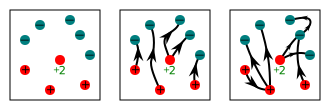
\includegraphics[width = \textwidth]{Boundaries/Path_endpoints/dot-to-dot}
\end{center}




\section{Closed loops}

Consider a multi-surface \(\mathbf{F}\). The boundary of surfaces have no endpoints, and are ``closed loops":
\[\nabla \bullet (\nabla \times \mathbf{F}) = 0\]    

If multi-path \(\mathbf{J}\) has no endpoints, then \(\mathbf{J}\) will be referred to as being a {\bf multi-loop}.

\[\mathbf{J} \quad\text{ is a multi-loop (closed loop) if and only if }\quad \nabla \bullet \mathbf{J} = 0\]

While the boundary of any multi-surface is a multi-loop, it is also the case that given an arbitrary multi-loop \(\mathbf{J}\), that there exists some multi-surface whose boundary is \(\mathbf{J}\):

\begin{thm}
If multi-path \(\mathbf{J}\) is such that \(\nabla \bullet \mathbf{J} = 0\) then there exists a multi-surface \(\mathbf{F}\) such that \(\nabla \times \mathbf{F} = \mathbf{J}\)
\end{thm}

This multi-surface \(\mathbf{F}\) can be created by filling each loop with a surface that has the correct orientation. This filling can be done by starting at a specific point on the loop, and then ``extending" a film be following the loop. The resultant multi-surface is {\bf not unique}, as there are infinitely many ways to fill a loop. The image below shows a multi-loop and two possible multi-surfaces whose boundaries are the given multi-loop. 

\begin{center}
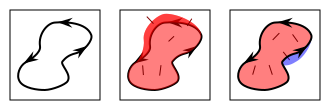
\includegraphics[width = \textwidth]{Boundaries/Surface_boundaries/surface_filling}
\end{center}

Below are examples of filling in more exotic loops with surfaces. On the left, there is the trefoil knot, while on the right, there is a helical coil. Helical coils have important applications in electronics and electromagnetism. 

\begin{center}
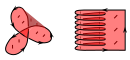
\includegraphics[width = 0.75\textwidth]{Boundaries/Surface_boundaries/exotic_surface_filling_examples}
\end{center}




\section{Closed surfaces}

Consider a multi-volume \(U\). The surfaces of volumes have no boundaries, and are ``closed surfaces/bubbles":
\[\nabla \times (\nabla U) = 0\]    

If multi-surface \(\mathbf{F}\) has no boundary, then \(\mathbf{F}\) will be referred to as being a {\bf multi-bubble}.

\[\mathbf{F} \quad\text{ is a multi-bubble (closed surface) if and only if }\quad \nabla \times \mathbf{F} = 0\]

While the surface of any multi-volume is a multi-bubble, it is also the case that given an arbitrary multi-bubble \(\mathbf{F}\), that there exists {\bf a unique} multi-volume whose surface is \(\mathbf{F}\):

\begin{thm}
If multi-surface \(\mathbf{F}\) is such that \(\nabla \times \mathbf{F} = 0\)
then there exists a {\bf unique} multi-volume \(U\) such that \(\nabla U = \mathbf{F}\)
\end{thm}

This multi-volume \(U\) can be created by filling each of the bubbles with a volume that has the correct weight (outwards oriented bubbles are filled with negative volume). The resultant multi-volume is {\bf unique}, as there is only one way to fill a bubble, unlike filling a boundary or connecting two points.



\begin{tabular}{cc}
\parbox{0.5\textwidth}{
Given a multi-loop \(\mathbf{J}\) and a multi-bubble \(\mathbf{F}\), the net number of times loop \(\mathbf{J}\) enters bubble \(\mathbf{F}\) is equal to the net number of times loop \(\mathbf{J}\) leaves bubble \(\mathbf{F}\). Entrance points have an equal and opposite weight to exit points. This means that the net total of all the intersection points is \(0\): \(\int \mathbf{J} \bullet \mathbf{F} = 0\). 

\begin{thm}
If multi-path \(\mathbf{J}\) is such that \(\nabla \bullet \mathbf{J} = 0\), 

and multi-surface \(\mathbf{F}\) is such that \(\nabla \times \mathbf{F} = 0\), 

then \(\int (\mathbf{J} \bullet \mathbf{F}) = 0\)
\end{thm}
} & \parbox{0.5\textwidth}{
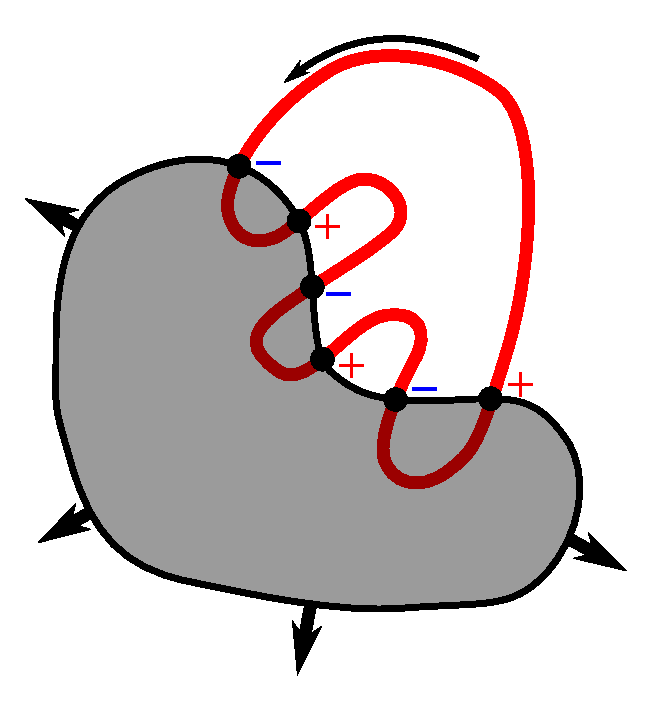
\includegraphics[width = 0.5\textwidth]{Intersections/Path-surface_intersections/closed_surface_and_closed_path}
}
\end{tabular}



\begin{tabular}{cc}
\parbox{0.5\textwidth}{
Consider a balanced multi-point \(\rho\) and a multi-bubble \(\mathbf{F}\). If \(\mathbf{J}\) is a multi-path whose endpoints are \(\rho\), then the net number of times \(\mathbf{J}\) intersects \(\mathbf{F}\) {\bf does not depend} on the choice of \(\mathbf{J}\). 

\begin{thm}
If multi-point \(\rho\) is such that \(\int \rho = 0\), 

and multi-surface \(\mathbf{F}\) is such that \(\nabla \times \mathbf{F} = 0\), 

and multi-paths \(\mathbf{J}_1\) and \(\mathbf{J}_2\) are two choices  
of multi-paths where \(\nabla \bullet \mathbf{J} = \rho\), 

then \(\int (\mathbf{J}_1 \bullet \mathbf{F}) = \int (\mathbf{J}_2 \bullet \mathbf{F})\)
\end{thm}

This is illustrated on the right where the two choices of paths result in the same net number of intersections with the bubble.
} & \parbox{0.5\textwidth}{
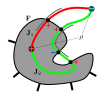
\includegraphics[width = 0.5\textwidth]{Intersections/Path-surface_intersections/closed_surface_and_different_paths}
}
\end{tabular}



\begin{tabular}{cc}
\parbox{0.5\textwidth}{
Consider two multi-loops \(\mathbf{J}\) and \(\mathbf{K}\). If \(\mathbf{F}\) is a multi-surface whose counterclockwise boundary is \(\mathbf{J}\), then the net number of times \(\mathbf{F}\) intersects \(\mathbf{K}\) {\bf does not depend} on the choice of \(\mathbf{F}\). 

\begin{thm}
If multi-path \(\mathbf{J}\) is such that \(\nabla \bullet \mathbf{J} = 0\), 

and multi-path \(\mathbf{K}\) is such that \(\nabla \bullet \mathbf{K} = 0\),

and multi-surfaces \(\mathbf{F}_1\) and \(\mathbf{F}_2\) are two choices
of multi-surfaces where \(\nabla \times \mathbf{F} = \mathbf{J}\), 

then \(\int (\mathbf{F}_1 \bullet \mathbf{K}) = \int (\mathbf{F}_2 \bullet \mathbf{K})\)
\end{thm}

This is illustrated on the right where the two choices of surfaces result in the same net number of intersections with the loop.
} & \parbox{0.5\textwidth}{
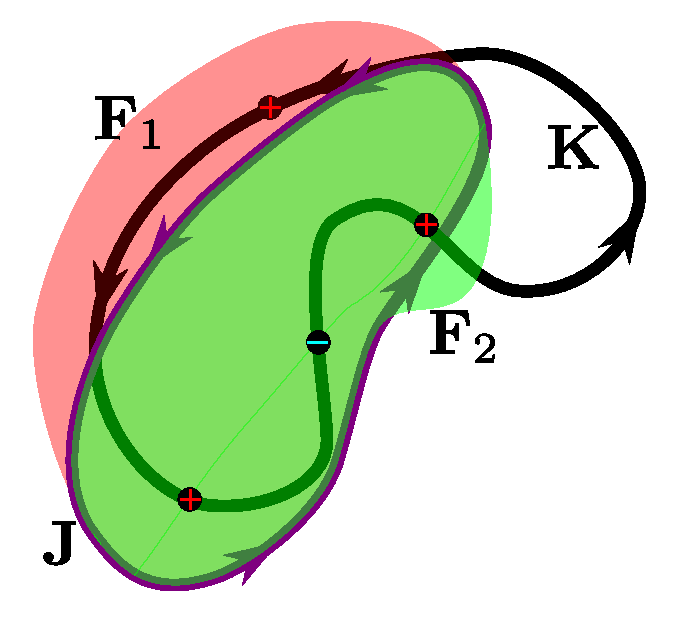
\includegraphics[width = 0.5\textwidth]{Intersections/Path-surface_intersections/closed_path_and_different_surfaces}
}
\end{tabular}